\documentclass{report}
\usepackage{graphicx}

\newcommand{\tab}{\hspace*{3em}}
\usepackage{enumerate}

\begin{document}

\title{Practical 1: PROMELA and SPIN}

\date{\parbox{\linewidth}{\centering%
\textsc{Student ID: 120017875}\endgraf
\textsc{Module: CS4052 Logic and Software Verification}\endgraf
\textsc{Lecturer: Juliana Bowles}\endgraf
\today}}
\maketitle

\section*{Part 1}
\tab The task is to write a PROMELA specificaton with processes Sender and Receiver. Sender transmits values from 1 to 10 to the Receiver.
However, values are not transmitted directly -- two intermediate processes Intermediate1 and Intermediate2 are used non-deterministically for this purpose. Both keep track of the total sum of values that they have transmitted.

\subsection*{Implementation}
\tab I have two slightly different implementations for this task. The first one implements what is asked for, while the second one is more experimental. First of them has four different processes -- Sender, Receiver, Intermediate1 and Intermediate2. All of them are defined as active (this means that they will be running in the initial system state). Communication between processes happens via channels. There are two channels for communication between Sender and intermediate processes (one for each) and a channel for communication between intermediate processes and Receiver. The process flow is as follows: 
\begin{itemize}
\item \textbf{Sender} looks at a global variable called \textit{value} (initially set to 1), and, if this is less than or equal to 10, Sender has two options -- either send this value via \textit{intermediate1} channel or via \textit{intermediate2} channel. For both options Sender also increments the \textit{value} variable. If \textit{value} is bigger than 10, Sender breaks out of the loop and terminates.
\item Meanwhile, \textbf{Intermediate1} and \textbf{Intermediate2} listen for incoming information using each their corresponding channel. Both of these processes also have global counters that keep track of the total sum of values that have gone through them. So once a message is received, its value is added to the corresponding counter and is then sent on to the receiver.
\item Finally, \textbf{Receiver} listens for incoming information and keeps track of how many values it has received. Once the number of values received equals 10, it breaks the listening loop and terminates.
\end{itemize}
\tab It is worth mentioning that all the integer variables here are of the type byte, as they can be larger than 2 (thus bit would not do), yet their values will never exceed 255, therefore byte is the most appropriate and space saving data type to use. It should also be pointed out that not all of the processes will terminate naturally -- the intermediate processes will be timed out, as they will keep listening after all of the values have been sent already. However, this does not affect the functionality.
\par My second implementation of the task is based on the fact that both intermediate processes described above have essentially the same method bodies. Therefore, instead of explicitly creating two different processes, I created two instances of the same Intermediate process. I also reduced the number of channels connecting Sender and intermediate processes to only one. Thus Sender deterministically sends values from 1 to 10 to this channel, and both instances of Intermediate listen to it. Non-determinism is present in the fact that any of the processes could get any of the messages. The one to get the message increments its counter and sends the message on to Receiver. Counters are still separate and global. A process knows which counter to increment depending on its process ID, which is unique.

\subsection*{Testing}
\tab The most obvious way of checking whether the specification has executed as expected is looking at the communication pattern produced by iSpin. It shows what process received and sent what values. I also checked whether the sum of the total numbers of values transmitted for both processes was 55 (sum of numbers from 1 to 10), and used print statements for debugging purposes.
\par It is more difficult to test the second implementation, as it does not directly comply to what was stated in the task. It is because indeterminism appears in the pattern of which process reads which value, rather than in the choice of the Sender. One way to check whether the results of both implementations are equally non-deterministic would be running both of them with a large number of different seeds, storing the results (the values got transmitted through each process) and checking whether both result sets come from the same distribution (the probability distribution of a specific value being transmitted via one or the other of the processes should be Binomial). However, from a brief inspection by running a few tests with different seed values, the second implementation seems equally non-deterministic as the first one.

\subsection*{Channel Capacities}
\tab I experimented with various channel capacities to see how they impact the behaviour of the specification. Here are my findings:
\begin{itemize}
\item It turns out that the order in which transmitting and receiving happens depends on the buffer size. When a channel capacity is chosen to be 0, there is no buffer. Thus sending and receiving have to be synchronised -- the value has to be read right after it has been sent, otherwise there is nowhere it can stay. See Figure 1. for an example of synchronous communication.
\par However, if the channel capacity is increased, there are more options for the order of reading/sending messages, as the messages sent can be held in a buffer and read later. See Figure 2. for an example of communication between processes where all channels have the capacity of 4, and messages get stored in the buffer before they are read.

\begin{figure} [\textwidth]
\hspace{0cm}
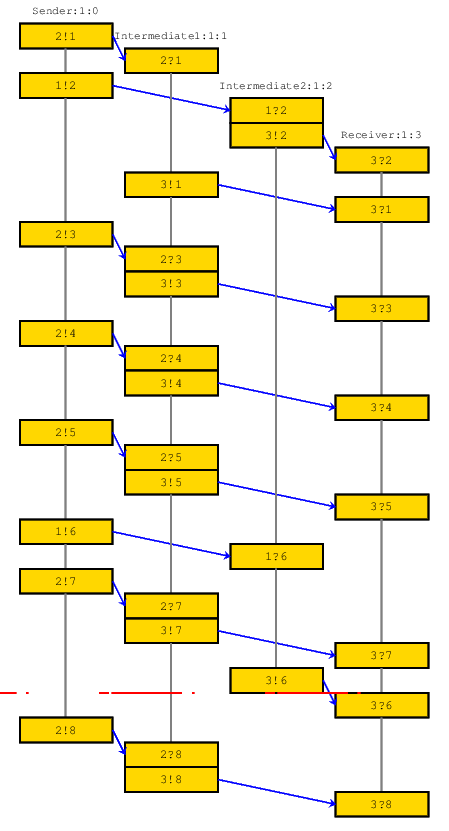
\includegraphics[scale=0.6]{Images/sync.png}
\caption{Synchronised communication using un-buffered channels. Reading takes place right after sending. (Number of values sent is decreased to 8 for illustration purposes.)}
\end{figure}

\begin{figure} [\textwidth]
\hspace{0cm}
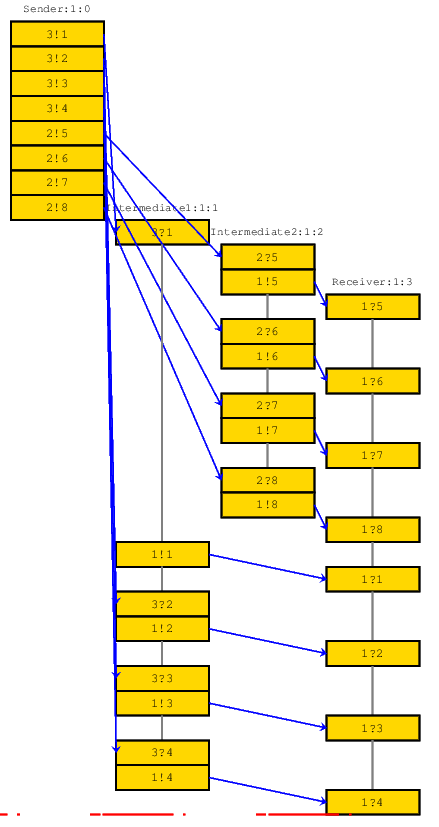
\includegraphics[scale=0.6]{Images/nonsync.png}
\caption{Here the buffer size has been set to 4 for all channels. It can be seen that messages are kept in buffer instead of being immediately after they have been sent. Intermediate1, for example, has values from 1 to 4 stored in the buffer until it decides to read them, while Intermediate2 has values from 5 to 8. (Number of values sent is decreased to 8 for illustration purposes.)}
\end{figure}

\item Channel capacity also impacts the possible order in which the Receiver gets values. For my implementation of the task, whenever the intermediate process reads a value, it must transmit it to the Receiver before listening for another value. Thus, in the case of no buffer, the order in which the Receiver gets the values might contain single values that are out of order, but no larger disorder is possible. See Figure 1., where 1 and 2, and 6 and 7 are swapped. It would also be possible to deliver a sequence like, say, 2,3,4,5,6,7,8,1 (here 1 is placed at the very end) or 2,3,4,1,5,7,8,6 (here 1 and 6 are displaced). This happens when Sender sends the first value to, say, Intermediate1, and the process reads it but does not send it on. Then the Sender sends a number of values to Intermediate2, which reads them and sends them on to the Receiver. And only then Intermediate1 sends its value, thus it arrives "with a delay". In other words, one of the intermediate processes holds back on a value. As there is no buffer, only one value can be held back at a time. It would not be possible, say, to deliver a sequence like 3,4,5,6,7,8,1,2, as Intermediate1 can not hold both -- 1 and 2. However, if the channel is buffered, it can hold back more than one value, as in Figure 2., where Intermediate1 holds back on 1, 2, 3 and 4. Thus the bigger the buffer, the more mixed up the resulting order can get.

\end{itemize}

\section*{Part 2}
\tab The aim of this task was to create N processes that all want to print infinitely often, and makes sure that only one process at a time is printing. The information about the processes that are currently printing is stored in a global boolean array \textit{print} -- if a process is printing the entry in the array corresponding to the process` ID is set to true. Formal verification should be used to test correctness of the solution.

\subsection*{Implementation}
\tab For the processes to communicate so that only one of them is printing at a time, either a global variable (a semaphore that would lock the critical printing section) or some explicit way of telling a specific process that it can now print is needed. I chose the second approach -- communicating via a shared channel named \textit{canPrint}. All the processes are listening to it, and the one that receives a message goes into the printing section. There it registers the fact that it is printing by updating the \textit{print} array and calculates how many processes are currently in the critical section by looping through the \textit{print} array and counting how many of its elements are positive. This value is stored as a global variable \textit{numOfPrintingP}. It then prints and sets the corresponding boolean element back to false. To initiate this process, one of the processes needs to send the first message. I used the fact that Spin assigns unique process IDs to each process and made process with the pid 0 the one to send the initial message.

\subsection*{Testing}
\tab To make sure that the implementation satisfies the condition that only one process is in the critical printing section at all times, I used a never claim. The never claim consists of a single do loop. It checks the value of \textit{numOfPrintingP}, if this value is bigger than one, the loop is broken, never claim terminates and the verifier flags it up as a violation.
\par The specification written does pass the verification with no errors. Figure 3. shows some of the results returned. It can be seen that the verifier has not been able to reach the end of the never claim (which is good) and of the process Pi. This is the case because Pi wants to print forever, therefore never terminates.
\par I also tried to break my never claim by setting an extra value of \textit{print} to true (print[1] = true), so that two processes would be registered as printing at the same time. This did indeed result in an error and verification not being passed, which is a good thing -- it means that the never claim reports the situations that should never occur.

\begin{figure} [\textwidth]
\hspace{0cm}
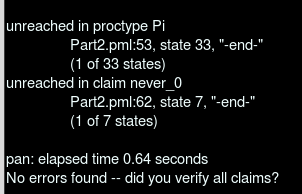
\includegraphics[scale=0.8]{Images/never.png}
\caption{Results of the verification of Task 2.}
\end{figure}

\section*{Part 3}
\tab This task asks to verify a set of requirements for the given specification, and to determine whether they should or should not hold within it, and whether weak fairness (every process that is constantly enabled from some point onwards should get its turn infinitely often) has an impact on the results. To do that, I firstly rewrote the requirements as linear temporal logic (LTL) formulae using atomic propositions that I defined. The following atomic propositions are used: \textit{xOdd} for x being odd, \textit{ySmallerEqualX} for y being smaller or equal to x, and \textit{yEqualsx} for x and y being equal. Here are the given requirements and my comments on them:
\begin{enumerate}[(a)]
\item \textbf{x is always odd.}

LTL formula: \texttt{ltl a \{[]xOdd\}}

This requirement does not hold for the given specification regardless of whether the fairness has been enforced. It makes sense, as any time P2 is executed, x changes its parity. Therefore, with or without fairness, there are execution sequences that lead to x changing from being odd to being even, and the requirement gets violated. When I tried to verify this LTL, Spin returned an error trail with one such execution fragment which firstly executed P3, and then went on to P2, thus making x=2 and violating the requirement (see Figure 4.).

\begin{figure} [\textwidth]
\hspace{0cm}
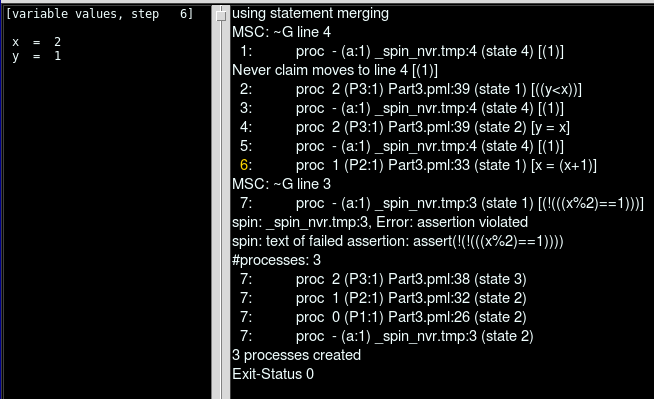
\includegraphics[scale=0.7]{Images/ltlA.png}
\caption{An error trail showing the requirement a) of task 3. being violated.}
\end{figure}

\item \textbf{It is possible that from a certain point onwards x is always odd.}

This requirement can not be directly rewritten in LTL, as LTL does not support possibility operators. However, we can write the opposite of the requirement in LTL: \texttt{ltl b \{[]<>!xOdd\}}. This formulae states that x will always infinitely often be even. If this was not always the case, then there would be a possibility of a point from which on x is never even, leading to the given requirement.

When verifying the opposite of the requirement, it turns out that it holds when weak fairness is enforced, but fails to hold without it. This is because without fairness the execution sequence can limit the number of times process P2 is given a go, as there is nothing that would force its execution, although it is constantly enabled. Thus the parity of x might not be changed from a certain point onwards and it might not be even infinitely often. However, when weak fairness is enforced, P2 is executed infinitely many times, and x gets to be even infinitely many times. Thus, as the opposite requirement holds with weak fairness and does not hold without it, it can be deduced that the given requirement will hold without fairness but not with it, which makes sense -- with no fairness it might so happen that x is odd from some point onwards and never changes its parity as P2 does not get a turn.

\item \textbf{It is possible that from a certain point onwards x is infinitely often odd.}

Once again, the requirement can not be directly expressed using LTL, therefore I look at its opposite: \texttt{ltl c \{[]<>[]!xOdd\}}. This formulae states that x will always eventually become and stay even. It is the opposite of the given requirement, as x becoming and staying even prevents it from being odd infinitely many times.

The opposite requirement does not hold for the given specification regardless of fairness being enforced or not. It is because it is not necessarily the case that x will eventually become and stay odd. It might happen (in the case of no fairness), but it is not guaranteed. Therefore the original condition holds with and without fairness -- it is always possible that x is infinitely often odd.

\item \textbf{It is always true that y $\leq$ x.}

LTL formula: \texttt{ltl d \{[]ySmallerEqualX\}}

This requirement does not hold for the given specification. This time it does not have anything to do with the fairness; the problem lies in data types and their behaviour -- when x reaches the upper limit of a byte (255), incrementing it will result in x being truncated back to 0. Meanwhile, y can stay at a higher value, resulting in x being less than y. An example of this can be seen in Figure 5. that shows the error trail returned by the verifier.

\begin{figure} [\textwidth]
\hspace{0cm}
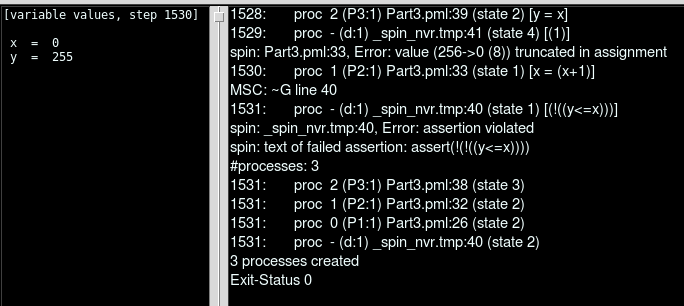
\includegraphics[scale=0.7]{Images/ltlD.png}
\caption{An error trail showing the requirement d) of task 3. being violated. x (a variable of a type byte) reaches value 255 and gets truncated back to 0 after the next increment, as it is exceeding the upper limit of byte.}
\end{figure}

\item \textbf{It is always true that when y=x it follows that at some point y$\neq$x.}

LTL formula: \texttt{ltl e \{[](yEqualsX->(<>!yEqualsX))\}}

This requirement holds for the given specification both, with and without weak fairness. In the case of enforced weak fairness, the reason for this is obvious -- all the processes are enabled, thus they are all given their turns, and, while P3 makes x=y, P1 and P2 lead to y$\neq$x. Thus x will be infinitely often equal and not equal to y. This should not necessarily be the result if fairness was not enforced -- P3 could be the only process to have a go, and x would constantly equal y (the only way to break the implication; if x never equals y the implication is vacuously true). However, P3 is defined so that it can only proceed when y is smaller than x, therefore P1 and/or P2 will also get a go, and the requirement holds. When y is smaller than x condition is removed, the requirement does not hold without fairness.

\end{enumerate}

\section*{Part 4}
\tab Spin (Simple Promela INterpreter) provides two main types of functionality -- simulation and verification. Simulation shows a single execution of the specification, which can be random, interactive or guided (when a specific trail is used). It is useful for illustrating how the processes work and interact, however, it does not give any information about what desired properties do or do not hold for the model. This is what the verifier is used for. In this section I will briefly describe the way in which PROMELA models are represented in Spin, LTL model checking algorithms, current limitations and mechanisms for making verification more efficient.

\subsection*{Underlying representation of PROMELA models}
\tab Spin uses finite state automaton to verify a given PROMELA model. Firstly, each PROMELA process is transformed into a finite state automaton. Then the process behaviour is modelled, also using finite state automata. One automaton is created per asynchronous process behaviour. Finally, all of this is gathered together in another automaton that now represents the global system behaviour \cite{Holzmann}. This resulting FSA can be referred to as "state-space" of the system, as it contains all of the different possible states in which the model can be. Each of these states contains a state vector -- a structure that holds information of the global variables and the state of each process, such as the value of its local variables \cite{lect}. This state space can be represented as a graph. When undergoing a verification, an exhaustive depth-first search on this graph is performed to examine all the possible execution sequences. This is how assertions and liveness properties are verified, and the "dead" states (the ones that are never reached) are found. The states that are seen during the examination are pushed on a depth-first stack. If an error occurs, the error-trail can be easily produced by going through this stack. Never claims take a bit of extra work -- they are converted into Buchi automata \cite{KP}. Never claims are executed after each "turn" made by another process, which on the automaton level means that for each transition made by the automaton representing the model, Buchi automaton also makes one. If the Buchi automaton reaches a final state, the never claim terminates -- an essential property has been violated and an error is returned.

\subsection*{LTL model checking algorithms}
\tab LTL formulae in PROMELA can always be expressed as never claims, thus they have the same underlying representation as described in the previous section -- Buchi automata. In Figure 6. a Buchi automata constructed using LTL e) from Task 3. can be seen. This LTL claims that whenever y equals x, there will be a point in the future where y does not equal x. This automaton is then executed step by step together with the main automaton. If processes terminate at a stage when the Buchi automaton is at state 1, an error will be thrown, as it is not an accepting state. Similarly, if an unbreakable loop leading from the state 1 back to 1 is registered, a violation of the property will be registered.

\begin{figure} [\textwidth]
\hspace{1cm}
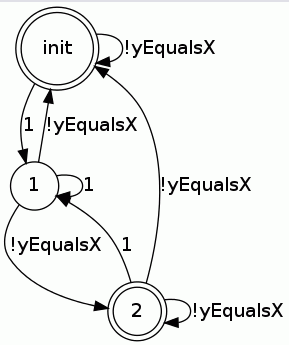
\includegraphics[scale=0.7]{Images/buchi.png}
\caption{A Buchi automaton created by the LTL e) from Task 3. Substitute number 1 by yEqualsX.}
\end{figure}

\subsection*{Mechanisms for improving scalability and efficiency}


\subsection*{Limitations}




Spin = Simple PROMELA Interpreter
formal verification of distributed and concurrent systems
(e.g. operating systems, data communications protocols)
Promela is suitable to describe concurrent systems:
dynamic creation of concurrent processes.
(synchronous/asynchronous) communication via message channels.

Simulation shows one execution.
random, interactive or guided.
not useful for finding bugs!

Verification checks every execution looking for a counterexample.
exhaustive or approximate verification of correctness properties.
a counterexample is a computation that violates a correct property

Simulation can detect assertion errors, but can't prove that there are no errors. That's where verifier comes in.

Nota Bene
When the search is bounded, Spin will not be exploring part of the system
statespace, and the omitted part may contain property violations that you
want to detect ⇒ you cannot assume that the system has no violations

Spin -- a simulator for Promela programs and a verifier for the properties of Promela programs.

The main part of Promela : placing claims on a program, that SPIN has
to verify !
Various types :
Basic assertions.
End-state labels.
Progress-state labels.
Accept-state labels.
Never claims.
Trace assertions.


 generates a C
program that performs an efficient verification of the protocol’s correctness properties.
 SPIN can perform an exhaustive
verification that can establish with mathematical certainty whether or not a given behavior
is error-free. To verify very large systems, it provides a “bit state storage” technique
known as supertrace that can collapse the state space to a small number of bits per
reachable state with minimal side-effect [4]. 

The executable program pan can now be executed to perform the verification. The verification is truly exhaustive: it tests all possible event sequences in all possible orders (Spin manual)

\begin{thebibliography}{9}

\bibitem{Holzmann}
  Gerard J. Holzmann,
  \emph{The Model Checker SPIN} from \emph{IEEE TRANSACTIONS ON SOFTWARE ENGINEERING} Vol. 23,
  1997, accessed on 21.10.2015 on http://spinroot.com/spin/Doc/ieee97.pdf
  
  \bibitem{KP}
  Ville R. Koskinen, Juha Plosila,
  \emph{Applications for the SPIN Model
Checker – A Survey}, Turku Centre for Computer Science
  2006
  
    \bibitem{lect}
   Matt Dwyer, John Hatcliff,
  \emph{Lecture SPIN-INTRO:
Introduction To SPIN} from the lecture series \emph{Specification and Verification of Reactive Systems}, Kansas State University,
  2001,  accessed on 21.10.2015 on http://spinroot.com/spin/Doc/SpinIntro.pdf

\end{thebibliography}

\end{document}